\section{Animación de la anatomía humana} 
\label{art:anatomy}


%\subsection{Introducción}

Una de las necesidades básicas que debe cubrir un simulador es poder mostrar información anatómica de pacientes virtuales con las que trabajará el usuario. En  \cite{preim2018survey} se explica la necesidad de que los estudiantes tengan un conocimiento profundo de la anatomía humana, estructuras, su posición relativa, variabilidad, etc. Es fundamental que un médico cuente con esos conocimientos previamente a la realización del entrenamiento médico.

Existen dos formas comúnmente utilizadas para representar modelos tridimensionales por computador. Lo más habitual es utilizar una malla poligonal, normalmente compuesta por triángulos o rectángulos (quads), comúnmente llamadas \ac{B-rep}. El principal inconveniente es que representa solo la superficie del modelo y no contiene información interna.  % \del{Esta malla generalmente está compuesta de polígonos llamados facetas o caras que son la unidad básica de un modelo tridimensional. Las caras más comunes son: triángulos, siendo este el polígono más simple; o rectángulos, que normalmente se descomponen en dos triángulos. El triángulo es la figura más utilizada debido a su menor complejidad matemática en los diferentes cálculos relacionados con la informática gráfica (interpolaciones, manejo de vecinos, etc.).}
%A lo largo del tiempo, las tarjetas gráficas se han diseñado con especial énfasis en el tratamiento de triángulos.
Por otra parte, existe otro tipo de representación, llamada volumétrica, que permite una representación visual completa de un objeto tanto del exterior como del interior, que la representación poligonal no era capaz. Sin embargo, esto produce una gran complejidad al intentarlas representar mediante técnicas de imagen generada por computador.
En la figura \ref{fig:HVP} se puede apreciar las dos representaciones del mismo modelo anatómico.

\begin{figure}[h]
   \centering
    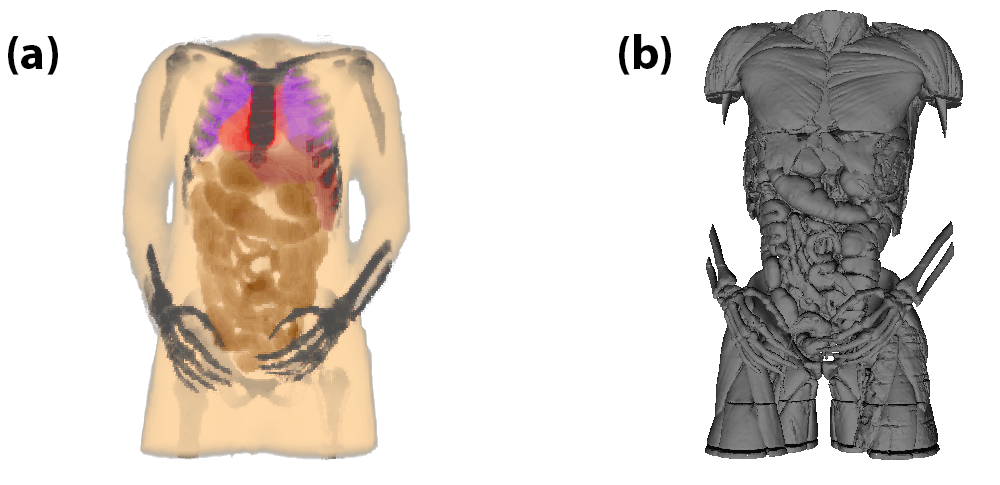
\includegraphics[width=0.5\textwidth]{IMG/volvsb-rep.png}
    \caption{La figura (a) muestra la representación volumétrica del \emph{Visible Human Project}\cite{ackerman1998visible}. La figura (b) muestra la malla poligonal del mismo modelo. }
   \label{fig:HVP}
\end{figure}
\todo{hace falta explciar la malla de tetraedros?}



Respecto a la representación de modelos anatómicos humanos, es fácil encontrar  varios modelos comerciales como puede ser: \emph{ZygoteBody}$^{TM}$ ~\cite{kelc2012zygote}, \emph{Anatomium} ~\cite{Anatomium},   \emph{BioDigital Human} \cite{qualter2012biodigital} o modelos como \emph{Visible body}\cite{visible2012visible} que solo está centrado en músculos y deformaciones predefinidas. Todos ellos representados como malla de polígonos. Estos modelos han sido  diseñados por artistas y representan cánones no realistas, además no reflejan fielmente la variabilidad anatómica de los pacientes a las que podría enfrentarse un médico. 

En la actualidad, existe una línea de investigación para llevar datos de pacientes reales a modelos virtuales y de esta forma usar datos capturados usando técnicas de imagen médica (como \ac{TC}, \ac{IRM} o \ac{US}). La base de datos de  \emph{Visible Human Project}\cite{ackerman1998visible} y  \emph{Segmented Inner Organs}\cite{VoxelMan} basado en el anterior, representan uno de los modelos volumétricos de prueba más utilizados en la búsqueda de métodos para extraer modelos virtuales procedentes de imágenes médicas \cite{ferrante2017slice}.

Tanto los modelos comerciales como los modelos obtenidos a través de imagen médica presentan el mismo problema: los modelos son presentados en una misma postura, que suele coincidir con la postura de adquisición. Esto hace que los datos de pacientes sean estáticos y limitados, por consiguiente, no representan la mayoría de los casos. En algunos procedimientos médicos como la artroscopia de rodilla o el bloqueo del nervio axilar, las imágenes capturadas no presentan la postura adecuada para el procedimiento. En el caso de la artroscopia, se necesita la rodilla flexionada frente a la habitual imagen capturada de la pierna extendida. En el caso del bloqueo del nervio, es necesario que el paciente se sitúe con el brazo en abducción de 90 grados respecto del tronco y el antebrazo en flexión de 90 grados en comparación a la mayoría de las imágenes médicas que son capturadas en una posición relajada. 

Es importante remarcar que la mayoría de las técnicas de registro entre imágenes médicas y modelos anatómicos tridimensionales que se presentan en \cite{ferrante2017slice} no son capaces de capturar adecuadamente todos y cada uno de los tejidos del paciente. En ocasiones solo se centran en tejidos concretos como puede ser la piel, huesos y músculos en general. Además, las técnicas actuales de imagen médica tampoco son capaces de recuperar las propiedades mecánicas de todos los tejidos, siendo esto un gran inconveniente si se requiere una descripción de todos los tejidos.

Por tanto, estos simuladores necesitarían un método que pueda tratar modelos virtuales con tejidos internos, completos o incompletos, y poder adaptar su postura al procedimiento a entrenar. Se busca poder utilizar una variabilidad de modelos, con el objetivo de que los usuarios puedan entrenar con el máximo número de pacientes virtuales del que se dispongan sin importar la posición con la que fueron creados.

Es importante hacer mención al trabajo de  \emph{Dicko et al.}~\cite{Ali2013}.  En este artículo, los autores han desarrollado un método para modelar la anatomía interna de un paciente virtual, transfiriendo los tejidos internos de un modelo anatómico de referencia como \emph{ZygoteBody}$^{TM}$~\cite{kelc2012zygote} a un modelo registrado a partir de una imagen médica. Con esta técnica, es posible registrar y modelar los tejidos internos de datos obtenidos de \ac{IRM}. Al igual que en las técnicas de registro, en esta publicación se citan ciertos problemas con la interpretación de los tejidos adiposos. Este trabajo se centra solo en el proceso de registro y modelado sin detallar el proceso de animación utilizado. Tampoco mencionan como se realiza la etapa de \emph{rigging} y la de pesado que se detallarán en la siguiente sección.  


En la siguiente sección, se presentarán una visión general de los diferentes algoritmos existentes para animar modelos tridimensionales de caracteres articulados. La animación consiste en deformar las representaciones superficiales 
\todo{quieres que utilice el termino b-rep?. Marcos. Solo cuando quede bien}
o volumétricas por medio de modelos matemáticos. Estas técnicas suelen ser clasificadas en dos tipos: aquellas que tienen en cuenta las propiedades físicas del modelo y aquellas que solo utilizan operaciones geométricas para animar el modelo. Actualmente, es habitual que los algoritmos geométricos estén orientados a ser interactivos (sacrificando deformaciones precisas desde un punto de vista físico físicamente correctas) frente a los algoritmos físicos centrados en una deformación más \del{realista} \new{plausible}. Aun así, existen algoritmos que combinan ambos enfoques para conseguir deformaciones más realistas con tasas interactivas, o reducir el tiempo de procesado mientras se mantiene el comportamiento físico. 


\subsection{Animación esqueletal}
\label{art:animation}
\label{art:virtualskel}

La animación esqueletal es un método geométrico que se utiliza para anima un modelo articulado representado por su malla superficial, gracias a un esqueleto virtual, asociando los vértices a los huesos virtuales. Esta técnica permite transferir el movimiento del esqueleto la representación superficial. Esta técnica fue introducida por N. Magnenat Thalmann en 1988 \cite{thalmann88} y sigue siendo la técnica más utilizada debido a su sencillez y su fácil implementación en el cauce gráfico actual. A pesar de la existencia de métodos más realistas, esta técnica se usa prácticamente en todos los sistemas de animación interactivos ya que simplifica el trabajo de los artistas (el número de grados de libertad del esqueloto virtual es mucho menor al numero de grados de liberta del la representación superficial) y es el paso previo a algoritmos más complejos. %Por ejemplo, se puede animar mediante captura de movimientos y cinemática inversa, entre otros.

La técnica se basa en una abstracción matemática, un esqueleto virtual, que se utiliza para definir los puntos de rotación de las \acl{joints} de los modelos. Este esqueleto se define como un conjunto de huesos virtuales jerarquizados y se encuentran conectados entre sí. La figura \ref{fig:virtualskeleton} muestra como un esqueleto virtual está superpuesto a un paciente virtual. Las esferas grises representan los centros de rotación de los \emph{\acs{joints}}, mientras que, los prismas representan la relación de herencia entre ellos. Estos huesos están pensados para que el artista dirija los movimientos del personaje y defina animaciones que la técnica de \emph{skinning} trasladará a la malla superficial según se define en \cite{thalmann88}. 

\begin{figure}[h]
   \centering
    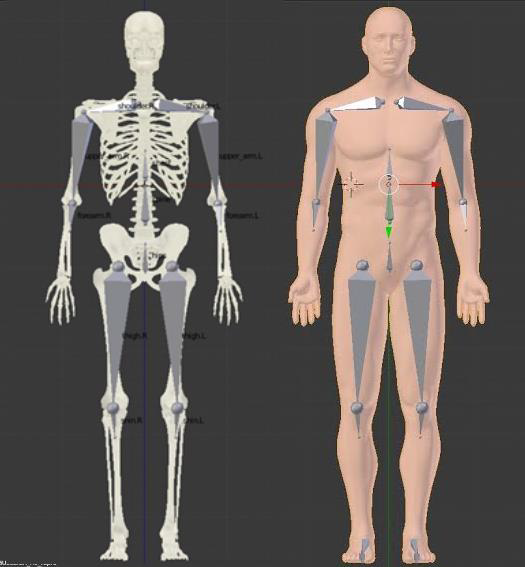
\includegraphics[width=0.5\textwidth]{IMG/virtualskeleton.png}
    \caption{Esqueleto virtual ajustado al tejido oseo de un modelo anatómico.}
   \label{fig:virtualskeleton}
\end{figure}

Con el paso del tiempo, esta técnica ha sido divida en fases que ayudan a definir el cauce de la animación esqueletal:

\begin{itemize}
    \item \emph{Rigging}\footnote{Término ampliamente utilizado para la creación o adaptación del esqueleto virtual}: En esta etapa se crea el esqueleto virtual específicamente para el modelo que se vaya a animar.
    \item Pesado: Una vez creados los huesos virtuales, se asigna el peso de influencia de cada hueso para cada vértice de la piel del modelo.
    \item \emph{Skinning}\footnote{Término ampliamente utilizado  para la transferencia de movimientos}: Se define los algoritmos que van a transferir el movimiento de los huesos virtuales a la malla superficial asociada. 
    \item Selección de poses: Se define un movimiento para los huesos que producen una deformación concreta al modelo superficial.
\end{itemize}

A continuación, se mostrará la revisión de la literatura existente para cada etapa. Se hará especial mención a aquellas técnicas automáticas.


\subsubsection{Rigging}
\label{art:rigging}

El proceso de \emph{rigging} consiste en crear un esqueleto virtual lo más cercano a el esqueleto original, que tuviera el modelo tridimensional que se está animando. Este trabajo normalmente es realizado por un artista ayudado de un programa de \ac{CAD} como puede ser \emph{Blender} \cite{blender} o \emph{3DS MAX} \cite{3ds}. 

Cuando se trata de animar modelos orgánicos, el uso de esqueletos virtuales, que solo se definen por rotaciones, presentan limitaciones al tener unos movimientos más complejos. Algunos trabajos intentan definir articulaciones basados en modelos anatómicos \cite{joints} con \emph{splines}\footnote{ Curva diferenciable definida en porciones mediante polinomios} mejorando así el movimiento del hueso, pero dificultando la creación del esqueleto virtual y el proceso de manipulación.

Existen algunos trabajos que tratan de automatizar el proceso de creación de esqueletos virtuales siguiendo dos enfoques: adaptando esqueleto predefinido \cite{huang2013robust} o infiriendo el esqueleto en base a la malla superficial \cite{jacobson2014part}.
Actualmente, se pueden encontrar varias propuestas para crear un esqueleto virtual automáticamente para cualquier modelo virtual ~\cite{borosan2012rigmesh,feng2014fast,avril2016animation}.





\subsubsection{Pesado}
\label{art:pesado}

Este proceso  determina cual es la influencia de cada hueso virtual en cada vértice de la malla superficial. El cálculo de esta influencia se denomina pesado, debido a que se calcula una serie de pesos $w_{i,j}$ que relacionan un vértice $i$ con el hueso $j$.
Para asegurar una deformación correcta, se presuponen las siguientes condiciones que se tienen que cumplir:
\begin{eqnarray}
%\begin{equation}
\label{cond1}
w_{i,j}\geq 0 \;\;\;\;\;\;\;\; \forall i \in V \wedge \forall j \in B   \\
%\end{equation}
%\begin{equation}
\label{cond2}
\sum_{j \in B} w_{i,j} = 1\ \;\;\;\;\;\;\;\;\;\;\;\;\;\;\;\;
\forall i \in V
%\end{equation}
\end{eqnarray}
donde $V$ es el conjunto de vértices de la malla poligonal y $B$ es el conjunto de huesos en el esqueleto virtual. No puede existir un hueso que influya negativamente a un vértice, por ello se tiene que cumplir la condición \ref{cond1}. Además, para garantizar que no se genere movimientos extras, es necesario cumplir la condición \ref{cond2}.
Por último, resulta intuitivo pensar que las transiciones entre huesos virtuales deberían ser progresivas, el gradiente de los pesos debe ser suave, para evitar efectos extraños y discontinuidades en la malla.

Originalmente, al igual que la etapa anterior, un artista era el encargado de realizar la tarea manualmente, donde se utilizaban herramientas \ac{CAD} para \emph{pintar} la influencia de un hueso en la malla superficial. Actualmente en la literatura se pueden encontrar métodos totalmente automáticos \cite{huang2013robust,pan2017automatic}. 
Algunos de estos trabajos no tienen en cuenta la conectividad de la malla y puede ser que haya vértices topológicamente lejanos con pesos similares. Es por eso, que se han propuesto soluciones como \cite{Baran:2007} utilizando la ecuación de \emph{Laplace} que ayudan a calcular transiciones más suaves en la malla. Aunque esta solución es más compleja (resolución de sistemas de ecuaciones, cálculo de vecindad, etc.), ofrece transiciones más realistas y menor intervención manual. Esta técnica está restringida a mallas superficiales que deben rodear completamente al esqueleto virtual.

Existen trabajos posteriores como el de \emph{Jacobson et al.}~\cite{Jacobson:2011}, donde se mejora la etapa de pesado para ser capaz de manejar puntos de anclaje (point handles, esta bien traducido?), huesos virtuales y cajas contenedoras. Se propone minimizar la energía \emph{Laplaciana} de las restricciones de los anclajes con el objetivo de conseguir una continuidad  de primer orden (Ec. \ref{eqn:1}):
\begin{equation}
\label{eqn:1}
\mathrm{arg\,min}_{W_j, j=1..m}\sum_{j}^m\frac{1}{2}\int_\Omega \left \|  \nabla W_j\right \|^2 dV,
\end{equation}
donde $W_j$ son los pesos del manejador $j$ y $m$ es el número de puntos de anclaje. 

\subsubsection{Skinning}
\label{art:skinning}

Esta etapa es la que define como se transfieren los movimientos de los huesos virtuales a los vértices que componen la malla superficial que los envuelve. Según la formulación matemática que desarrolle la ecuación de \emph{skinning} (Ec. \ref{eqn:skinning}), se han creado distintos métodos como \ac{LBS}, \ac{DQS} o \ac{SBS}.

\begin{equation}
\label{eqn:skinning}
v'_{i} = \sum_{j \in B} w_{i,j}f(\theta_{j},v_{i}) 
\end{equation}
Esta ecuación determina como calcular la nueva posición del vértice $v'_{i}$ de la malla. $\theta$ representa el movimiento de cada hueso $j$ del conjunto de huesos $B$ y $w_{i,j}$ su peso asociado a ese vértice. De esta forma, la nueva posición del vértice se calcula en función de la influencia del movimiento de cada hueso.

La técnica más habitual es \ac{LBS} presentada en \cite{thalmann88}, que se basa en calcular la nueva posición interpolando linealmente las matrices de transformación ($T$) de cada hueso virtual (Ec. \ref{eqn:LBS}).
\begin{equation}
\label{eqn:LBS}
v'_{i} = \sum_{j \in B} w_{i,j}T_{j}v_{i}
\end{equation}

\ac{LBS} sufre problemas debido a que la interpolación de las rotaciones se realiza de manera lineal. Esto lleva asociado efectos no deseados como: el colapso de la malla  en rotaciones(\emph{collapsed elbow}) o en giros (\emph{candy wrapper}). En la literatura, se pueden encontrar numerosas propuestas \cite{rumman2016state} pero normalmente llevan asociadas un incremento del coste computacional, o la aparición de otros artefactos no deseados. Uno de los métodos más populares es la técnica propuesta por \emph{Kavan et al.} en \cite{Kavan2008}, llamada \ac{DQS}, que intenta solventar las limitaciones de \ac{LBS} al utilizar la interpolación de cuaterniones duales (Ec. \ref{eqn:DQS}). Además, esta técnica se caracteriza por ser computacionalmente equivalente a \ac{LBS}. Aunque \ac{DQS} funciona bien en la mayoría de los casos, en el algún escenario produce que la malla se deforme en exceso. Visualmente resulta en una ganancia de volumen significativa (\emph{bulging}). 

\begin{equation}
\label{eqn:DQS}
v'_{i} = (\sum_{j \in B} DQ_{j}w_{i,j}) v_{i}
\end{equation}

Otras soluciones se han presentado como \emph{Lee et al.}~\cite{Lee2013}, que describe una técnica que se encarga de resolver los problemas de \ac{DQS} cuando se realizan escalados y cizallados, movimientos muy habituales en cine de animación pero algo infrecuente en modelos anatómicos.

En trabajos más recientes, \emph{Le y Hodgins}~\cite{le2016real} presentan una técnica que calcula unos nuevos \acl{COR} para cada vértice de la malla. Este enfoque solventa el problema de \emph{bulging} sin incrementar el coste computacional y no sufre del defecto \emph{candy wrapper}. El único inconveniente es la necesidad de un proceso previo para calcular todos esos nuevos centros.
%\todo{pongo el algoritmo de cor?}
% \begin{eqnarray}
% \label{eqn:COR}
% R = normalize( w_{i,1}q_{1} + w_{i,2}q_{2} + . . . + w_{i,b}q_{b})\\
% t = R_{LBS}c_{i} + t_{LBS} - Rc_{i} \\
% v'_{i} =  R_{q}v_{i} + t
% \end{eqnarray}

\todo{pongo imágenes de comparación?}

%
%
No es habitual que estos métodos tengan en cuenta la resolución contactos entre vértices de la malla. En \cite{Vaillant:2014}, se propone una solución geométrica con tasas interactivas que puede solucionar las auto colisiones. \emph{Vaillant et al.} calculan un campo escalar para cada hueso. Los vértices serán influenciados por el valor de cada campo escalar. Sin embargo, ese método no está pensado para animar modelos que representen tejidos óseos. Estructuras rígidas como los huesos se ven afectados por una función de suavizado, que se traduce en producir deformaciones no realistas. %16k de vertices 50 fps nosotros 1.5kk



\subsubsection{Selección de poses} 
\label{art:poses}
Esta etapa consiste en crear las animaciones  y los movimientos de los huesos virtuales que serán aplicadas a la malla superficial.   

Al igual que etapas anteriores, es habitual que estas animaciones sean creadas por artistas profesionales. Con la ayuda de las herramientas \ac{CAD}, los animadores definen el movimiento de los huesos virtuales en fotogramas clave y el software calcula la interpolación de los fotogramas intermedios. Estas herramientas también incluyen algoritmos de cinemática inversa \cite{Shi:2007}, que permiten al usuario posicionar el actuador final (hueso situado en un nivel inferior de la jerarquía) y calcular la posición del resto de articulaciones superiores. 
Además, la técnica de \ac{MoCap} está muy presente en los estudios cinematográficos. Los movimientos realizados por un actor son capturados a través de unas balizas situadas en los trajes que se utilizan. Estos puntos característicos permiten el registro de la posición y rotación que serán trasladados al esqueleto virtual \cite{Menache:1999}. En contraste con las grandes producciones, es posible utilizar un \ac{tracker} como Microsoft Kinect, para la animación de personajes virtuales \cite{Liu:2018}.


\subsection{Animación basada en modelos físicos}
\label{art:fisica}

Alternativamente a los métodos geométricos, los algoritmos basados en modelos físicos buscan simular el comportamiento real. Desde el trabajo seminal de \emph{Terzopoulos et al.}\cite{terzopoulos1987elastically}, la simulación física ha tomado una enorme importancia para crear los efectos como la elasticidad de la piel, el comportamiento del tejido graso o el comportamiento de los músculos con el objetivo de generar animaciones que puedan ser usadas en cine, simuladores médicos o para el estudio de la biomecánica. 

Inicialmente, se utilizaban métodos basados en la ley de elasticidad de \emph{Hooke} como se puede ver en los trabajos \cite{russell93,wilhelms1995modeling}, pero en la última década, han ido surgiendo cada vez más modelos biomecánicos y músculo-esquelético. Algunos de los modelos biomecánicos son creados manualmente para una parte específica de la anatomía humana ~\cite{Lee2009}. \emph{Patterson et al.} \cite{Patterson2012} consiguen simular el comportamiento muscular pero su técnica requiere de una etapa manual larga y tediosa, normalmente realizada por un experto. De manera similar, \emph{Fan et al.}~ \cite{Fan2014} describe una técnica capaz de simular el músculo preservando su volumen. El modelo anatómico puede ser generado a partir de imágenes médicas siempre y cuando se capturen del músculo relajado y la pose final. 

Aunque se pueden encontrar técnicas que recuperan los modelos músculo-esqueléticos de imágenes médicas \cite{blemker2007, gilles2010, schmid2009}, estos no suelen ejecutarse en tiempos interactivos, siendo necesario también propiedades mecánicas. Esta información no siempre se encuentra disponible. Hay que destacar que las técnicas citadas solo se centran en la simulación de los músculos y esqueleto, sin tomar en consideración otro tipo de tejidos.

Se pueden encontrar artículos que combinan métodos kinemáticos y dinámicos con el objetivo de conseguir tasas interactivas.  \emph{Ichim et al.} \cite{Ichim:2016} utilizan animaciones precalculadas (\emph{blendshapes}) en el contexto de animación facial. Las \emph{blendshapes} permiten un control directo y eficiente mientras que el modelo basado en físicas proporciona respuestas ante colisiones, tratamiento de la incompresibilidad y otros efectos dinámicos y colaterales. Lamentablemente, este enfoque no está adecuado a la animación de personajes. 


\emph{Kadlecek et al.}~\cite{kadlecek-16-reconstructing} presentan un método para crear modelos anatómicos preparados para deformaciones basadas en físicas. A partir del trabajo de \emph{Dicko et al.}\cite{Ali2013} proponen un cauce automático de reconstrucción a través de múltiples capturas preservando la estructura ósea. Aun así, en ciertas ocasiones, los autores observaron que algunos huesos sobresalían entre los músculos. Se debe remarcar que, aunque esta técnica permite simular inercias y movimientos colaterales, este trabajo no permite tasas interactivas.   % En comparación con nuestro método, utilizan tetraedros que contienen más de un tejido, mientras en el algoritmo propuesto los tejidos óseos generan sus propios tetraedros que sirven de condición de contorno en el calculo de la etapa de pesado.

\emph{Rumman and Fratarcangeli}~\cite{abu2015position} han propuesto un método inspirado en el algoritmo de deformación basado en el cálculo de las posiciones, omitiendo la velocidad y la aceleración (PBD Point-Based Dynamics \cite{Bender:2014}). Este trabajo permite animar cualquier personaje articulado gracias a la discretización del interior del modelo, permitiendo también animar los tejidos internos. Sin embargo, el alto coste computacional requiere de mallas en baja resolución para su ejecución en tiempos interactivos.

%se podría hablar de métodos basados en ejemplos 
%tengo un par de surveys donde podría sacar más paper
